\chapter{Hexadecimal to Seven-Segment Converter}
\label{HexToSeven}
\graphicspath{ {./Lab02HexToSeven/Fig} }


\hypertarget{objective}{%
\section{Objective }
\label{hex2Seven:objective}}

The objective of this lab is to become familiar with the always
statement used to implement truth tables, how to combine bits into
vectors and how to download synthesized code onto the development board.

Today's laboratory will require to learn about two new Verilog concepts,
The Always statement and Vectors. Let's look at the easier of these two,
Vectors, first.

\subsubsection{Vectors}

A vector is simply a collection of bits, very similar to an array in a
regular programming language. You might use a vector to represent a
3-bit binary number that you want to perform an operation on. There are
three things that you will need to know about vectors in order to
complete today's lab (and future labs), combining bits into a vector,
defining a vector, and accessing the bits of a vector. These operations
are illustrated in Figure~\ref{fig:combinVector}.

\begin{figure}[ht]
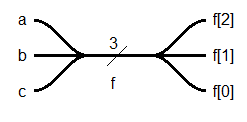
\includegraphics{image1.png}
\caption{A schematic illustration of combining bits into a vector, f,
and then accessing the individual bits of f.}
\label{fig:combinVector}
\end{figure}

Let's explore these ideas with the code snipped show in Listing~\ref{listing:vectorManipulation}. 
In this code snipped, the line of code assign f = \{a,b,c\}; combines the
individual signals a, b and c into a 3-bit vector. The left-most signal
in the parenthesis list becomes the MSB of the vector and the right-most
becomes LSB. In other words, \emph{a} is the MSB and \emph{c} the LSB.
Combining signals is more commonly called concatenation. You can
concatenate any arrangement of signals as long as the number of bits
comes out the same as the signal on the left-hand-side of the = sign.


\begin{lstlisting}[language=Verilog,
 caption={Verilog code which illustrates vector manipulations and declarations.},
 label={listing:vectorManipulation},
 frame=single]
module unimportantModuleName();

    wire a, b, c, x;			// Just some plain old wires
    wire [2:0] f, g, h;			// 3-bit vectors

    assign f = {a,b,c};			// Concatenate bits to vector
    assign g = {f[0], f[2:1]};		// re-arrange bits

    assign x = (f[0] & f[1]) ^ f[2];	// vectors are made of bits
    assign h = 3b'010;			// A constant vector to h
\end{lstlisting}

The statement wire {[}2:0{]} f; is how you define a vector. The numbers
in the square brackets are the indices of the most and least significant
bits of the vector. We will always index our vectors starting at 0, so
the highest index will always be one less than the number of elements in
the vector.

The statement assign x = (f{[}0{]} \& f{[}1{]}) \^{} f{[}2{]}; shows how
you can access the individual bits of a vector. While I am not sure what
the Verilog programmer was going for in this statement, you can access
the individual bit of a vector by putting the index of that bit in
square brackets. You can also access sub-vector by putting indices in
square brackets separated by a colon.

You can provide a constant value to a vector, an operation we will call
hardcoding, using the 3b'010; notation. The first number, 3, is the
length of the vector, b' means that this is a bit vector and the 010 is
the 3-bit value.

\subsubsection{Always}

We will use the Verilog \emph{always} statement to implement a function
using its truth table. Listing~\ref{listing:3in3outVerilog} shows an always statement that uses the
value of a signal x to compute the value of f.

\begin{lstlisting}[language=Verilog,
 caption={A 3-input, 3-output function realized with an always statement.},
 label={listing:3in3outVerilog},
 frame=single]
    wire [2:0] x;
    reg [2:0] f;
    
    always @(*)
        case (x)
            3'b000: f = 3'b000;
            3'b001: f = 3'b000;
            3'b010: f = 3'b000;
            3'b011: f = 3'b000;
            3'b100: f = 3'b000;
            3'b101: f = 3'b000;
            3'b110: f = 3'b000;
            3'b111: f = 3'b000;
        endcase
\end{lstlisting}

For the time being, we will trust that the statement always @(*)allows
the code between case and endcase to run continuously and concurrent
with any other statements in the module. Yes, this means that all the
code between case and endcase acts like a single assign statement. A
case statement uses the argument to case (in this case x) as a selector
for one of the rows below. Every possible value of x must be present and
when that value matches x, the action to the right of the colon is
performed. When we use a case statement as shown in Listing~\ref{listing:3in3outVerilog} 
you must make the output type reg.

All signals are either wire or reg type. A wire is a signal that has a
value provided to it by some active element. This active element might
be a gate or the output of a module. If a signal does not have an
explicit gate or module driving its value, it needs to be typed reg.

\hypertarget{part-1-combine-lab-1-functions.}{%
\section{Combine lab 1
functions.}\label{part-1-combine-lab-1-functions.}}

Let's explore vectors and the always statement by combining the three
functions created in last weeks assignment into one function.

\begin{enumerate}
\def\labelenumi{\arabic{enumi}.}
\item
  Go back to your Lab 01 solutions and extract the truth tables for
  function f04, f03, and f02. Put these values into the truth table
  shown in Table~\ref{table:combinedLab01}.
\end{enumerate}

\begin{longtable}[]{@{}
  >{\raggedright\arraybackslash}p{(\columnwidth - 10\tabcolsep) * \real{0.1667}}|
  >{\raggedright\arraybackslash}p{(\columnwidth - 10\tabcolsep) * \real{0.1667}}|
  >{\raggedright\arraybackslash}p{(\columnwidth - 10\tabcolsep) * \real{0.1667}}|
  >{\raggedright\arraybackslash}p{(\columnwidth - 10\tabcolsep) * \real{0.1667}}|
  >{\raggedright\arraybackslash}p{(\columnwidth - 10\tabcolsep) * \real{0.1667}}|
  >{\raggedright\arraybackslash}p{(\columnwidth - 10\tabcolsep) * \real{0.1667}}@{}}
\caption{The Truth Table for the combinedLab01 function. This
function has a 3-bit input and 3-bits output.}\tabularnewline
\toprule()
\begin{minipage}[b]{\linewidth}\raggedright
a
\end{minipage} & \begin{minipage}[b]{\linewidth}\raggedright
b
\end{minipage} & \begin{minipage}[b]{\linewidth}\raggedright
C
\end{minipage} & \begin{minipage}[b]{\linewidth}\raggedright
f04
\end{minipage} & \begin{minipage}[b]{\linewidth}\raggedright
f03
\end{minipage} & \begin{minipage}[b]{\linewidth}\raggedright
f02
\end{minipage} \\
\midrule()
\endfirsthead
\toprule()
\begin{minipage}[b]{\linewidth}\raggedright
a
\end{minipage} & \begin{minipage}[b]{\linewidth}\raggedright
b
\end{minipage} & \begin{minipage}[b]{\linewidth}\raggedright
C
\end{minipage} & \begin{minipage}[b]{\linewidth}\raggedright
f04
\end{minipage} & \begin{minipage}[b]{\linewidth}\raggedright
f03
\end{minipage} & \begin{minipage}[b]{\linewidth}\raggedright
f02
\end{minipage} \\ 
\midrule()
\endhead
0 & 0 & 0 & & & \\ \hline
0 & 0 & 1 & & & \\ \hline
0 & 1 & 0 & & & \\ \hline
0 & 1 & 1 & & & \\ \hline
1 & 0 & 0 & & & \\ \hline
1 & 0 & 1 & & & \\ \hline
1 & 1 & 0 & & & \\ \hline
1 & 1 & 1 & & & \\
%\bottomrule()
\label{table:combinedLab01}
\end{longtable}

\begin{enumerate}
\def\labelenumi{\arabic{enumi}.}
\item
  Create \textbf{a new project} folder within your \emph{lab2} directory
  called \emph{combinedLab01.}
\item
  Download \emph{combinedLab01.v} and \emph{combinedLab01}\_tb.v from
  Canvas to the project directory.
\item
  Create a project for these two files using the steps from last week's
  lab. 
\item
  Modify \emph{combinedLab01.v} so that \emph{combinedLab01} outputs the
  values given in Table~\ref{table:combinedLab01}.
\item
  Modify \emph{combinedLab01\_tb.v} so that \emph{combinedLab01} is run
  through every combination of inputs. Assert the inputs in increasing
  binary numbering order starting from 0,0,0 and going to 1,1,1.
\item
  Perform simulation using this test bench using the steps from last
  week's lab. 
  
\item
  \protect\hypertarget{CombinedLab01_Waveform}{}{}Capture the output
  waveform from Simulink. It should look something like the following.

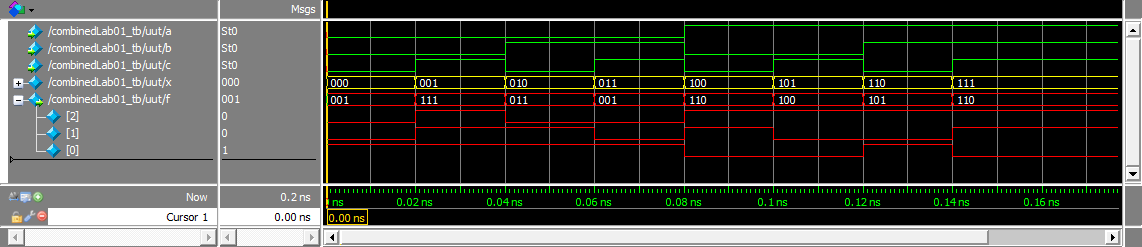
\includegraphics{image2.png}

\item
  From the information in the timing diagram, produce a truth table.
  Compare the truth table generated from the data in the timing 
  diagram to that you generated in Table~\ref{table:combinedLab01}.
\end{enumerate}

\subsubsection{Bridging the divide between logical and physical}

The process of converting your Verilog code to a form which you will
download onto the development board is called \emph{synthesis}. In order
to synthesize your Verilog code, you need to tell the Quartus software
which pins of the FPGA are associated with the ports in your top-level
Verilog module. In order to perform this assignment, you need to know
which pins of the FPGA are associated with useful hardware on the
development board. The engineers who created the development board made
the assignment of hardware components to FPGA pins when they laid out
the printed circuit board. These same engineers documented their
decisions in the Cyclone V GX Kit User Manual posted on the class web
page.

The Figure~\ref{fig:simpleVerilogDownload} shows a Verilog module called \emph{combinedLab01}
synthesized and downloaded into an Altera FPGA on the development board.
Note that ports a, b and c are connected to FPGA pins that are driven to
slide switches. Ports f{[}2{]}, f{[}1{]} and f{[}0{]} are connected to
FPGA pins that drive LEDs. In this way, a user can provide input to the
\emph{combinedLab01} module by moving the slide switches and observe the
circuit's output on the LEDs.

\begin{figure}[ht]
\caption{A simple Verilog design synthesized and downloaded onto the development board.}
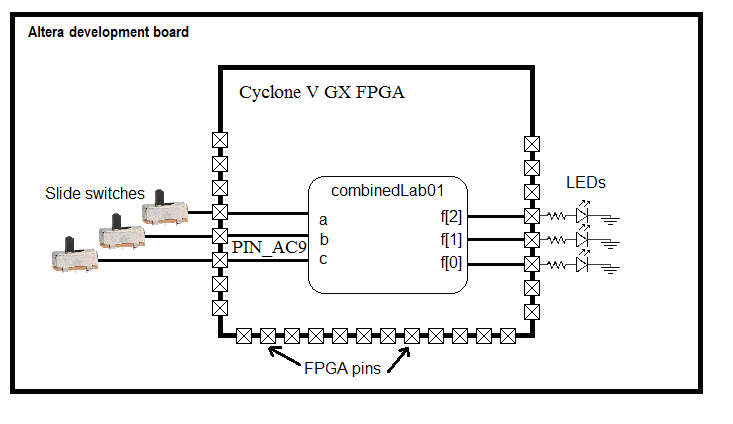
\includegraphics{image3.png}
\label{fig:simpleVerilogDownload}
\end{figure}

The development board contains an Altera Cyclone V GX FPGA. This FPGA
has many pins and they are identified by a lettered group and number.
For example, in Figure~\ref{fig:simpleVerilogDownload} port c of 
the combinedLab01 module is mapped to pin AC9.

You will need to be able to figure out the remaining pin assignments on
your own. To do this open up the User Manual posted on the class Canvas
page. Go to page \textbf{32} of the User Manual and find Table 3-3. It
shows that slide switch SW{[}0{]} is connected to PIN\_AC9.

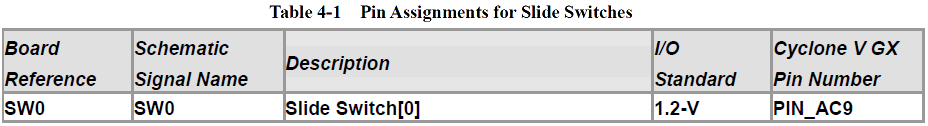
\includegraphics{image4.png}

The LEDs shown in figure 4-9 in the User Manual are active high, meaning
that the LED is active (illuminates) when you send it a high signal
(logic 1). Clearly, sending the LED a logic 0 turns the LED off. You can
place the slide switches in one of two positions (up or down). In the up
position, they assert a logic 1 on their input pin. Down causes the
slide switch to assert a logic 0 on its input pin.

Use the information to complete the pin assignment in 
Table~\ref{table:pinAssignmentCombinedLab01}.  We 
will use this assignment in the next section.

\begin{longtable}[]{@{}
|  >{\raggedright\arraybackslash}p{(\columnwidth - 12\tabcolsep) * \real{0.1429}}|
  >{\raggedright\arraybackslash}p{(\columnwidth - 12\tabcolsep) * \real{0.1428}}|
  >{\raggedright\arraybackslash}p{(\columnwidth - 12\tabcolsep) * \real{0.1428}}|
  >{\raggedright\arraybackslash}p{(\columnwidth - 12\tabcolsep) * \real{0.1428}}|
  >{\raggedright\arraybackslash}p{(\columnwidth - 12\tabcolsep) * \real{0.1429}}|
  >{\raggedright\arraybackslash}p{(\columnwidth - 12\tabcolsep) * \real{0.1430}}|
  >{\raggedright\arraybackslash}p{(\columnwidth - 12\tabcolsep) * \real{0.1430}}|@{}}
\caption{\protect\hypertarget{CombinedLab01_Pin_assignment}{}{}
Pin Assignment Table for combinedLab01.}\tabularnewline
\toprule()
\begin{minipage}[b]{\linewidth}\raggedright
Port
\end{minipage} & \begin{minipage}[b]{\linewidth}\raggedright
a
\end{minipage} & \begin{minipage}[b]{\linewidth}\raggedright
b
\end{minipage} & \begin{minipage}[b]{\linewidth}\raggedright
c
\end{minipage} & \begin{minipage}[b]{\linewidth}\raggedright
f{[}2{]}
\end{minipage} & \begin{minipage}[b]{\linewidth}\raggedright
f{[}1{]}
\end{minipage} & \begin{minipage}[b]{\linewidth}\raggedright
f{[}0{]}
\end{minipage} \\ \hline
\midrule()
\endfirsthead
\toprule()
\begin{minipage}[b]{\linewidth}\raggedright
Port
\end{minipage} & \begin{minipage}[b]{\linewidth}\raggedright
a
\end{minipage} & \begin{minipage}[b]{\linewidth}\raggedright
b
\end{minipage} & \begin{minipage}[b]{\linewidth}\raggedright
c
\end{minipage} & \begin{minipage}[b]{\linewidth}\raggedright
f{[}2{]}
\end{minipage} & \begin{minipage}[b]{\linewidth}\raggedright
f{[}1{]}
\end{minipage} & \begin{minipage}[b]{\linewidth}\raggedright
f{[}0{]}
\end{minipage} \\ \hline
\midrule()
\endhead
Signal name & SW{[}2{]} & SW{[}1{]} & SW{[}0{]} & LEDR{[}2{]} &
LEDR{[}1{]} & LEDR{[}0{]} \\ \hline
FPGA Pin No. & & & PIN\_AC9 & & & \\
\bottomrule()
\label{table:pinAssignmentCombinedLab01}
\end{longtable}

\subsubsection{Synthesizing a Verilog Module}

It's time to realize the \emph{combinedLab01} Verilog file to FPGA. To
do this follow these steps:

\begin{enumerate}
\def\labelenumi{\arabic{enumi}.}
\item
  In Project Navigator pane, select the File tab
\item
  Right mouse click \emph{combinedLab01.v} and select Set As Top Level
  Entity.
\item
  Processing -\textgreater{} Start -\textgreater{} Start Analysis and
  Elaboration
\item
  Assignments -\textgreater{} Pin Planner
\item
  In the Pin Planner pop-up you should see the pin assignment pane at
  the bottom of the window.

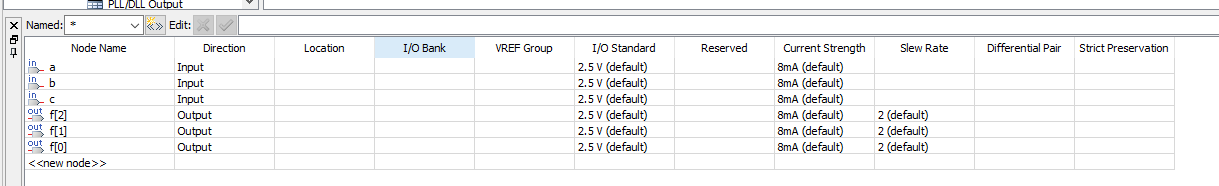
\includegraphics{image5.png}

\item
  Double click in the Location cell for row c
\item
  Scroll down the list of pins to PIN\_AC9
\item
  Complete the pin assignment for the other 5 inputs and outputs using
  the information contained in pin assignment table completed earlier.
\item
  Double check your pin assignments.
\item
  File -\textgreater{} Close. Note closing your file incorporates this
  assignment into the project.
\item
  Back in the Quartus window, Processing -\textgreater{} Start
  Compilation \textless Ctrl-L\textgreater{}
\item
  Tools -\textgreater{} Programmer
\item
  In the Programmer pop-up window click Add File\ldots{}
\item
  In the Select Programming File pop-up, navigate to your project
  directory, then into the output files folder, the select
  combinedLab01.sof, click Open. You should see something like the
  following.
  
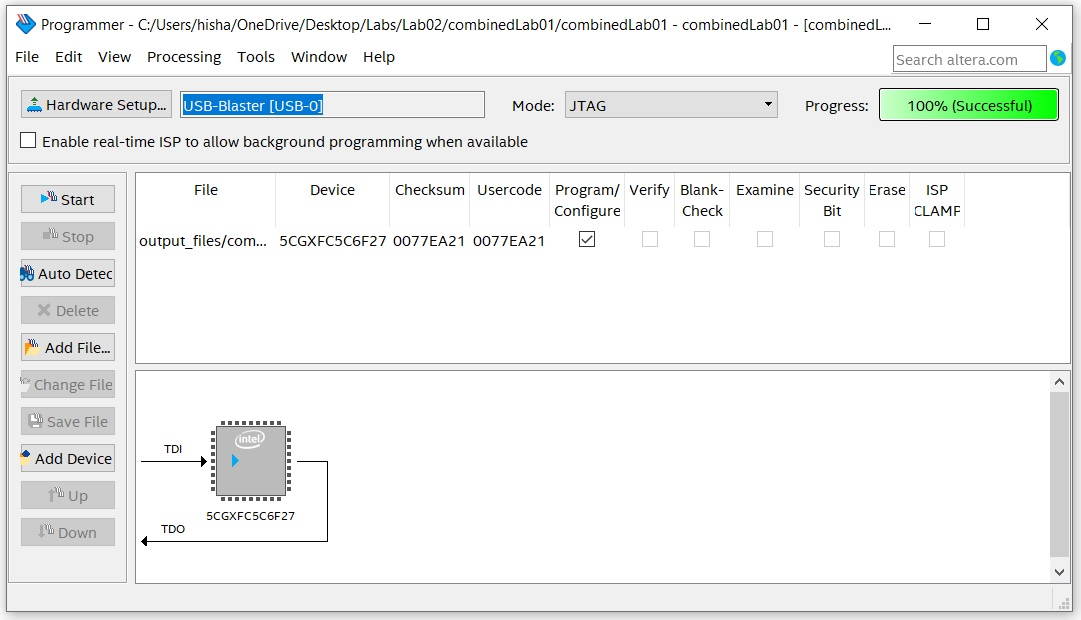
\includegraphics{image6.png}

\item
  Connect the Altera Cyclone V GX FPGA to your computer through the USB
  port, connect the power supply, and push the red power-on button. Try
  not to be annoyed by the infernal blinking LEDs.
\item
  In the Programmer pop-up

  \begin{enumerate}
  \def\labelenumii{\alph{enumii}.}
  \item
    Click Hardware Setup\ldots.
  \item
    In the Hardware Setup select USB-Blaster {[}USB=0{]} from the
    Currently selected hardware pull-down
  \item
    Click Close
  \end{enumerate}
\item
  Back in the Programmer window, the box next to Hardware Setup\ldots{}
  should reflect your choice. Click Start,
\item
  The Development board should stop its infernal blinking and run your
  program. You may notice that the unused LEDs are dimly illuminated.
\end{enumerate}

\begin{figure}[ht]
\caption{The development board properly configured and running the
combinedLab01 Verilog file.}
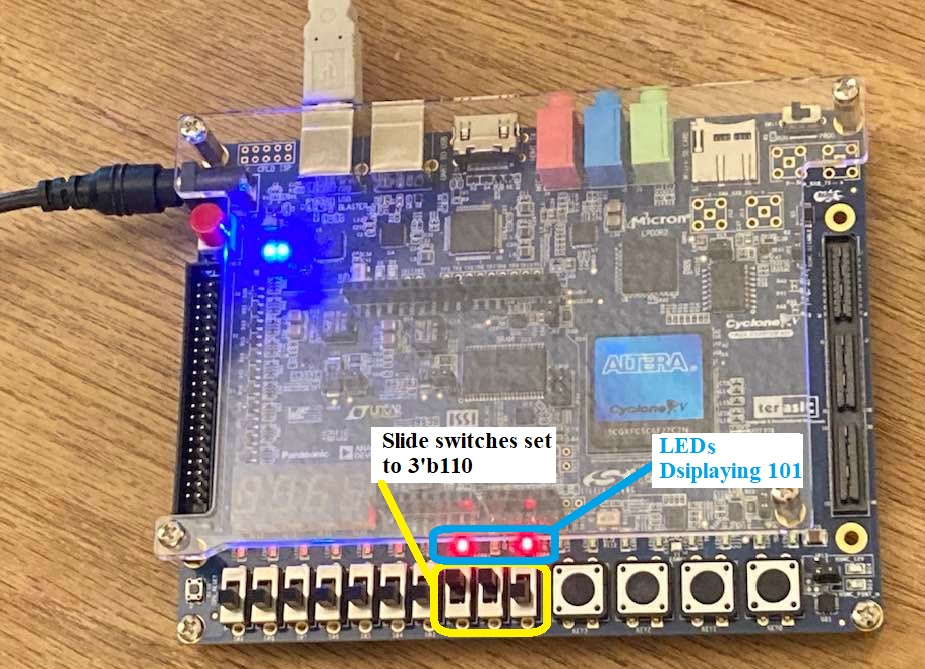
\includegraphics{image7.png}
\label{fig:combinedBoard}
\end{figure}

\hypertarget{part-2-hexadecimal-to-7-segment-converter}{%
\section{Hexadecimal to 7-segment
Converter}\label{part-2-hexadecimal-to-7-segment-converter}}

While working on the previous problem, you probably noticed that the
development Board has four 7-segment display. These figure 8 shaped
blocks above the slide switches are the devices which light up numbers
on some cash registers. We will be using these 7-segment displays for a
variety of purposes during the term, so it would be a good idea.

The hexadecimal-to-seven-segment-decoder is a combinational circuit that
converts a hexadecimal number to an appropriate code that drives a
7-segment display the corresponding value. \uline{BEWARE, the LEDs in
the 7-segment displays on the Development Board are active low,
asserting a logic 0 on the pin attached to a segment will cause that
segment to illuminate.}

\begin{figure}[ht]
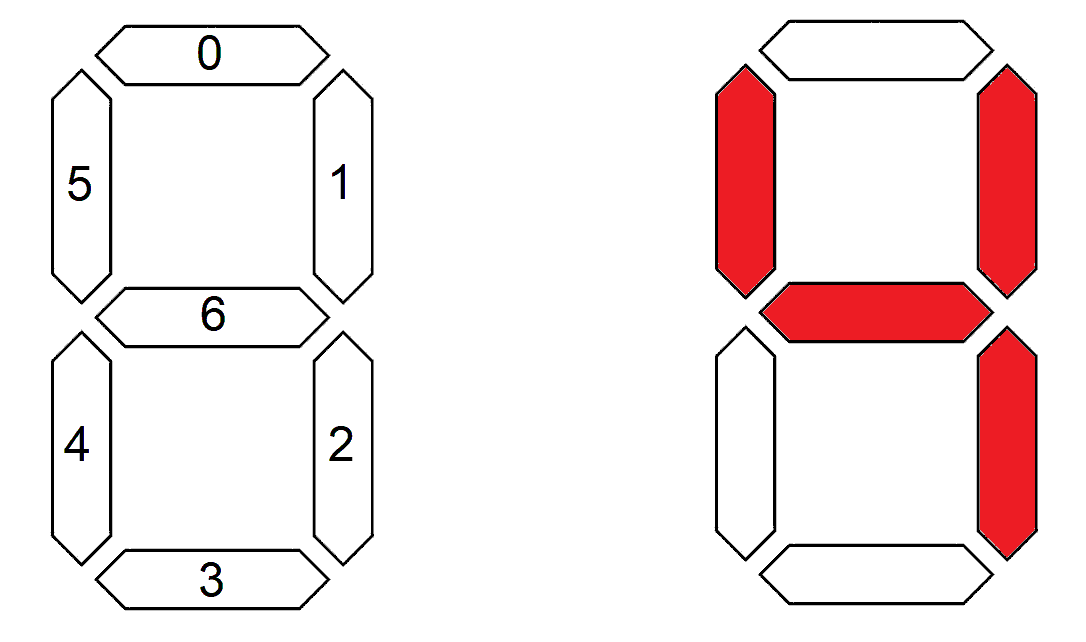
\includegraphics[width=0.5\paperwidth]{image8.png}
\caption{Left, the proper numbering of the segments. Right,
illuminating segments to form the number 4.}
\label{fig:sevenSeg}
\end{figure}

The pattern of segments to be illuminated for each digit is shown in
Figure~\ref{fig:sevenSeg}. For example, to display `4 output would be:

\begin{verbatim}
seg{[}6{]}=0 seg{[}5{]}=0 seg{[}4{]}=1 seg{[}3{]}=1 seg{[}2{]}=0
seg{[}1{]}=0 seg{[}0{]}=1

or seg = 7'b0011001
\end{verbatim}

Figure~\ref{fig:sevenSegChars} shows the proper formatting for all the values between 0 -- f.

\begin{figure}
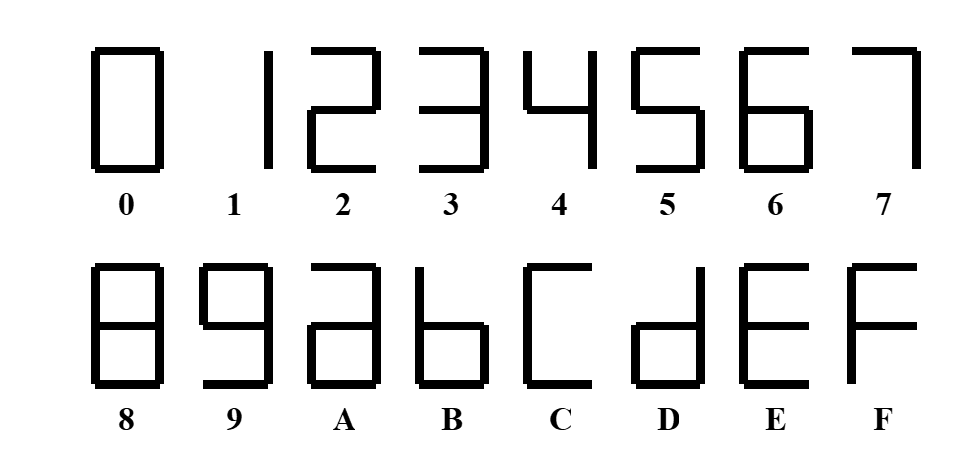
\includegraphics{image9.png}
\caption{The proper arrangement of LEDs to form hexadecimal characters.}
\label{fig:sevenSegChars}
\end{figure}

Figure~\ref{fig:hex2SevenSeg} shows the Verilog module you will be building in this lab - a
circuit that converts a 4-bit input, representing a hexadecimal value,
into the binary values to illuminate a 7-segment display with active low
LEDs.

\begin{figure}
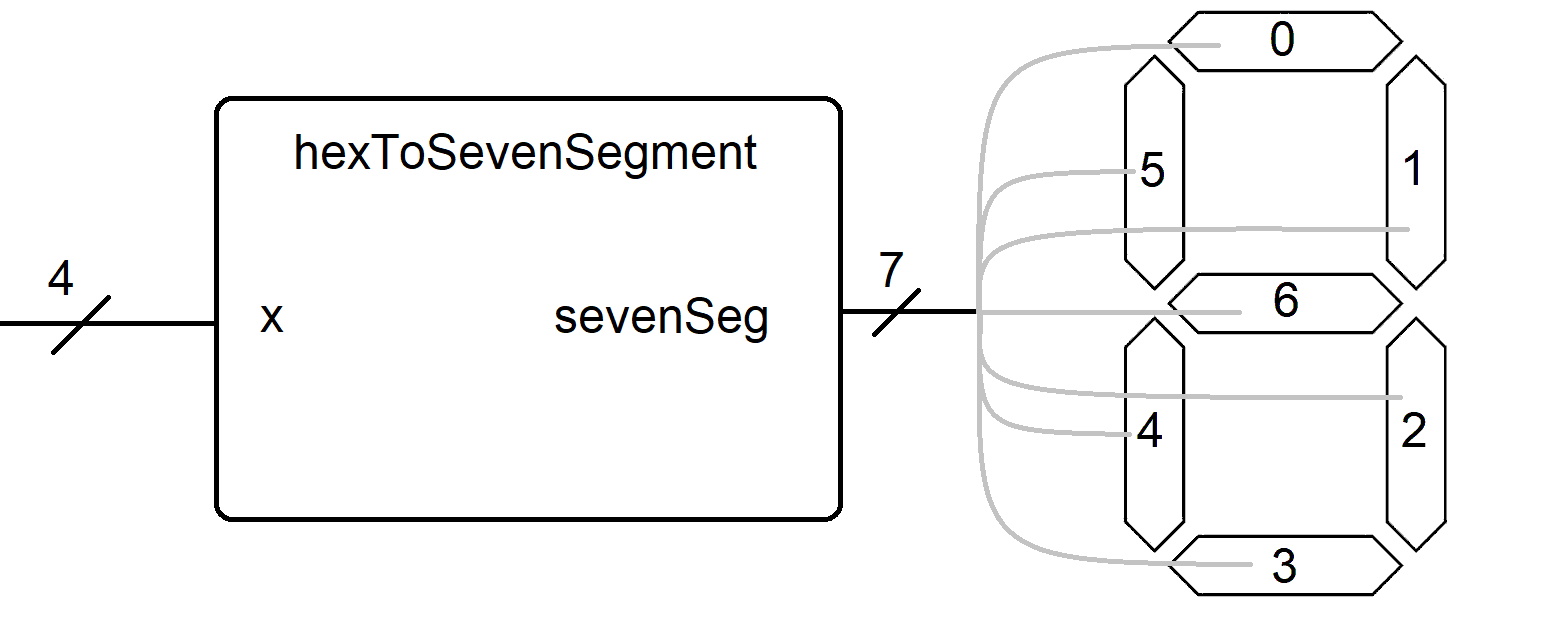
\includegraphics{image10.png}
\caption{The hexToSevenSeg Verilog module driving a 7-segment display.}
\label{fig:hex2SevenSeg}
\end{figure}

\begin{enumerate}
\def\labelenumi{\arabic{enumi}.}
\item
  Complete the Table~\ref{table:hex2sevenTruthTable} to illuminate the active low led segments
  to generate proper hexadecimal characters. I've renamed the sevenSeg
  output ``seg'' in the following table in order to make everything fit
  nicely.
\end{enumerate}

\begin{longtable}[]{@{}
  >{\raggedright\arraybackslash}p{(\columnwidth - 14\tabcolsep) * \real{0.1241}}|
  >{\raggedright\arraybackslash}p{(\columnwidth - 14\tabcolsep) * \real{0.1252}}|
  >{\raggedright\arraybackslash}p{(\columnwidth - 14\tabcolsep) * \real{0.1251}}|
  >{\raggedright\arraybackslash}p{(\columnwidth - 14\tabcolsep) * \real{0.1251}}|
  >{\raggedright\arraybackslash}p{(\columnwidth - 14\tabcolsep) * \real{0.1251}}|
  >{\raggedright\arraybackslash}p{(\columnwidth - 14\tabcolsep) * \real{0.1251}}|
  >{\raggedright\arraybackslash}p{(\columnwidth - 14\tabcolsep) * \real{0.1252}}|
  >{\raggedright\arraybackslash}p{(\columnwidth - 14\tabcolsep) * \real{0.1252}}@{}}
\caption{\protect\hypertarget{Hex2Seven_TruthTable}{}{}Truth
table or the hexToSevenSeg component.}\tabularnewline
\toprule()
\begin{minipage}[b]{\linewidth}\raggedright
x
\end{minipage} & \begin{minipage}[b]{\linewidth}\raggedright
seg{[}6{]}
\end{minipage} & \begin{minipage}[b]{\linewidth}\raggedright
seg{[}5{]}
\end{minipage} & \begin{minipage}[b]{\linewidth}\raggedright
seg{[}4{]}
\end{minipage} & \begin{minipage}[b]{\linewidth}\raggedright
seg{[}3{]}
\end{minipage} & \begin{minipage}[b]{\linewidth}\raggedright
seg{[}2{]}
\end{minipage} & \begin{minipage}[b]{\linewidth}\raggedright
seg{[}1{]}
\end{minipage} & \begin{minipage}[b]{\linewidth}\raggedright
seg{[}0{]}
\end{minipage} \\ \hline
\midrule()
\endfirsthead
\toprule()
\begin{minipage}[b]{\linewidth}\raggedright
x
\end{minipage} & \begin{minipage}[b]{\linewidth}\raggedright
seg{[}6{]}
\end{minipage} & \begin{minipage}[b]{\linewidth}\raggedright
seg{[}5{]}
\end{minipage} & \begin{minipage}[b]{\linewidth}\raggedright
seg{[}4{]}
\end{minipage} & \begin{minipage}[b]{\linewidth}\raggedright
seg{[}3{]}
\end{minipage} & \begin{minipage}[b]{\linewidth}\raggedright
seg{[}2{]}
\end{minipage} & \begin{minipage}[b]{\linewidth}\raggedright
seg{[}1{]}
\end{minipage} & \begin{minipage}[b]{\linewidth}\raggedright
seg{[}0{]}
\end{minipage} \\ \hline
\midrule()
\endhead
0000 & & & & & & & \\ \hline
0001 & & & & & & & \\ \hline
0010 & & & & & & & \\ \hline
0011 & & & & & & & \\ \hline
0100 & 0 & 0 & 1 & 1 & 0 & 0 & 1 \\ \hline
0101 & & & & & & & \\ \hline
0110 & & & & & & & \\ \hline
0111 & & & & & & & \\ \hline
1000 & & & & & & & \\ \hline
1001 & & & & & & & \\ \hline
1010 & & & & & & & \\ \hline
1011 & & & & & & & \\ \hline
1100 & & & & & & & \\ \hline
1101 & & & & & & & \\ \hline
1110 & & & & & & & \\ \hline
1111 & & & & & & & \\
\bottomrule()
\label{table:hex2sevenTruthTable}
\end{longtable}

Complete the pin assignment tables for the inputs and outputs of the 
hexadecimal to seven segment converter given in
Table~\ref{table:pinAssignmentHex2Seven}.

\begin{longtable}[]{@{}
  >{\raggedright\arraybackslash}p{(\columnwidth - 8\tabcolsep) * \real{0.1999}}|
  >{\raggedright\arraybackslash}p{(\columnwidth - 8\tabcolsep) * \real{0.1999}}|
  >{\raggedright\arraybackslash}p{(\columnwidth - 8\tabcolsep) * \real{0.2001}}|
  >{\raggedright\arraybackslash}p{(\columnwidth - 8\tabcolsep) * \real{0.1999}}|
  >{\raggedright\arraybackslash}p{(\columnwidth - 8\tabcolsep) * \real{0.2001}}@{}}
\caption{\protect\hypertarget{Hex2Seven_PinAssignment}{}{}Pair
of pin assignment tables for the hexToSevenSeg
component.}\tabularnewline
\toprule()
\begin{minipage}[b]{\linewidth}\raggedright
Port
\end{minipage} & \begin{minipage}[b]{\linewidth}\raggedright
x{[}3{]}
\end{minipage} & \begin{minipage}[b]{\linewidth}\raggedright
x{[}2{]}
\end{minipage} & \begin{minipage}[b]{\linewidth}\raggedright
x{[}1{]}
\end{minipage} & \begin{minipage}[b]{\linewidth}\raggedright
x{[}0{]}
\end{minipage} \\ \hline
\midrule()
\endfirsthead
\toprule()
\begin{minipage}[b]{\linewidth}\raggedright
Port
\end{minipage} & \begin{minipage}[b]{\linewidth}\raggedright
x{[}3{]}
\end{minipage} & \begin{minipage}[b]{\linewidth}\raggedright
x{[}2{]}
\end{minipage} & \begin{minipage}[b]{\linewidth}\raggedright
x{[}1{]}
\end{minipage} & \begin{minipage}[b]{\linewidth}\raggedright
x{[}0{]}
\end{minipage} \\ \hline
\midrule()
\endhead
Signal name & SW{[}3{]} & SW{[}2{]} & SW{[}1{]} & SW{[}0{]} \\ \hline
FPGA Pin No. & & & & PIN\_AC9 \\
\bottomrule()
\label{table:pinAssignmentHex2Seven}
\end{longtable}

\begin{longtable}[]{@{}
  >{\raggedright\arraybackslash}p{(\columnwidth - 14\tabcolsep) * \real{0.1083}}|
  >{\raggedright\arraybackslash}p{(\columnwidth - 14\tabcolsep) * \real{0.1431}}|
  >{\raggedright\arraybackslash}p{(\columnwidth - 14\tabcolsep) * \real{0.1431}}|
  >{\raggedright\arraybackslash}p{(\columnwidth - 14\tabcolsep) * \real{0.1431}}|
  >{\raggedright\arraybackslash}p{(\columnwidth - 14\tabcolsep) * \real{0.1341}}|
  >{\raggedright\arraybackslash}p{(\columnwidth - 14\tabcolsep) * \real{0.1095}}|
  >{\raggedright\arraybackslash}p{(\columnwidth - 14\tabcolsep) * \real{0.1095}}|
  >{\raggedright\arraybackslash}p{(\columnwidth - 14\tabcolsep) * \real{0.1095}}@{}}
\toprule()
\begin{minipage}[b]{\linewidth}\raggedright
Port
\end{minipage} & \begin{minipage}[b]{\linewidth}\raggedright
sevenSeg{[}6{]}
\end{minipage} & \begin{minipage}[b]{\linewidth}\raggedright
sevenSeg{[}5{]}
\end{minipage} & \begin{minipage}[b]{\linewidth}\raggedright
sevenSeg{[}4{]}
\end{minipage} & \begin{minipage}[b]{\linewidth}\raggedright
sevenSeg{[}3{]}
\end{minipage} & \begin{minipage}[b]{\linewidth}\raggedright
sevenSeg{[}2{]}
\end{minipage} & \begin{minipage}[b]{\linewidth}\raggedright
sevenSeg{[}1{]}
\end{minipage} & \begin{minipage}[b]{\linewidth}\raggedright
sevenSeg{[}0{]}
\end{minipage} \\ \hline
\midrule()
\endhead
Signal name & HEX0{[}6{]} & HEX0{[}5{]} & HEX0{[}4{]} & HEX0{[}3{]} &
HEX0{[}2{]} & HEX0{[}1{]} & HEX0{[}0{]} \\ \hline
FPGA Pin No. & & & & & & & \\ \hline
\bottomrule()

\end{longtable}
Now you are ready to write the Verilog code for the hexadecimal to seven
segment converter, assign pins to the inputs and outputs, and synthesize
and download the module to the development board.


\begin{enumerate}
\item
  Create \textbf{a new project} folder within your \emph{lab2} directory
  called \emph{hexToSevenSeg.}
\item
  Download \emph{hexToSevenSeg.v} and \emph{hexToSevenSeg \_tb.v} from
  Canvas to the project directory.
\item
  Create a project for these two files.
\item
  \protect\hypertarget{Hex2Seven_Verilog}{}{}Complete the case statement
  for \emph{hexToSevenSeg.v}
\item
  Modify \emph{hexToSevenSeg \_tb.v} so that \emph{hexToSevenSeg} is run
  through every combination of inputs. Assert the inputs in increasing
  binary numbering order starting from 0,0,0,0 and going to 1,1,1,1.
\item
  Perform simulation using this test bench as described in previous
  steps. You will need to ``run 100'' several times to go through all
  the inputs.
\item
  \protect\hypertarget{Hex2Seven_Waveform}{}{}Save this waveform as an
  image as done in the previous section. If the waveform is missing, you
  can add it back in using View -\textgreater{} Waveform.
\item
  From the information in the timing diagram, produce a truth table for
  \emph{hexToSevenSeg}.
\item
  Synthesize your design, bask in the glow of another success.
\end{enumerate}

\begin{figure}[ht]
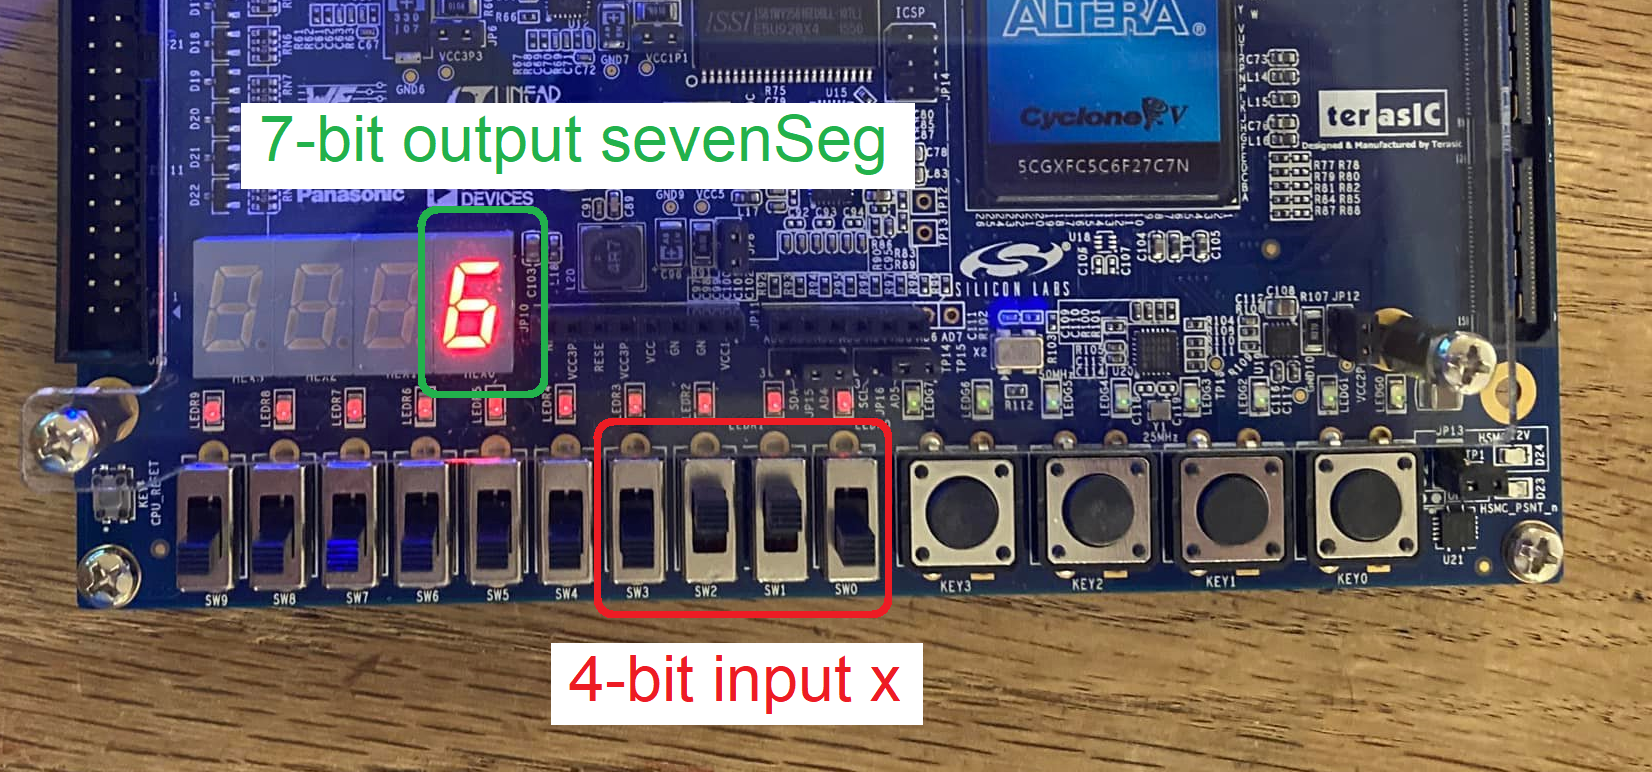
\includegraphics{image11.png}
\caption{The development board properly configured and running the hexToSevenSegment Verilog file.}
\end{figure}

\hypertarget{turn-in}{%
\section{Turn in:}\label{turn-in}}

Make a record of your response to numbered items below and turn them in
a single copy as your team's solution on Canvas using the instructions
posted there. Include the names of both team members at the top of your
solutions. Use complete English sentences to introduce what each of the
following listed items (below) is and how it was derived.

\subsubsection{Combine lab 1} 
\begin{itemize}
\item \protect\hyperlink{CombinedLab01_Waveform}{Link} Truth Table for combinedLab01 function 
(Table~\ref{table:combinedLab01})
\item \protect\hyperlink{CombinedLab01_Waveform}{Link} Timing diagram for combinedLab01 function
\item \protect\hyperlink{CombinedLab01_Pin_assignment}{Link} Pin assignment for combinedLab01 
(Table~\ref{table:pinAssignmentCombinedLab01})
\end{itemize}

\subsubsection{Hexadecimal to 7-segment}
\begin{itemize}
\item \protect\hyperlink{Hex2Seven_TruthTable}{Link} Truth Table for hexToSevenSeg function 
(Table~\ref{table:hex2sevenTruthTable})
\item \protect\hyperlink{Hex2Seven_Verilog}{Link} Verilog code for hexToSevenSeg function -- just the always/case statement
\item \protect\hyperlink{Hex2Seven_Waveform}{Link} Timing diagram for hexToSevenSeg function
\item \protect\hyperlink{Hex2Seven_PinAssignment}{Link} Pin assignment tables for hexToSevenSeg 
(Tables~\ref{table:pinAssignmentHex2Seven})
\item Demonstrate working hexadecimal to seven segment module on development board.
\end{itemize}


